\subsection{A* Search with heuristic}
\noindent The A* algorithm is a widely used technique for pathfinding and graph traversal. It relies heavily on heuristics to estimate the future cost of reaching the goal. Essentially, A* extends uniform cost search by incorporating a heuristic function to guide its path selection, making it more efficient in many cases. The choice of heuristic depends on the specific problem domain, highlighting the importance of domain knowledge. For A* to be consistent, the modified cost function must always remain greater than zero.

\begin{figure}[H]
	\centering
	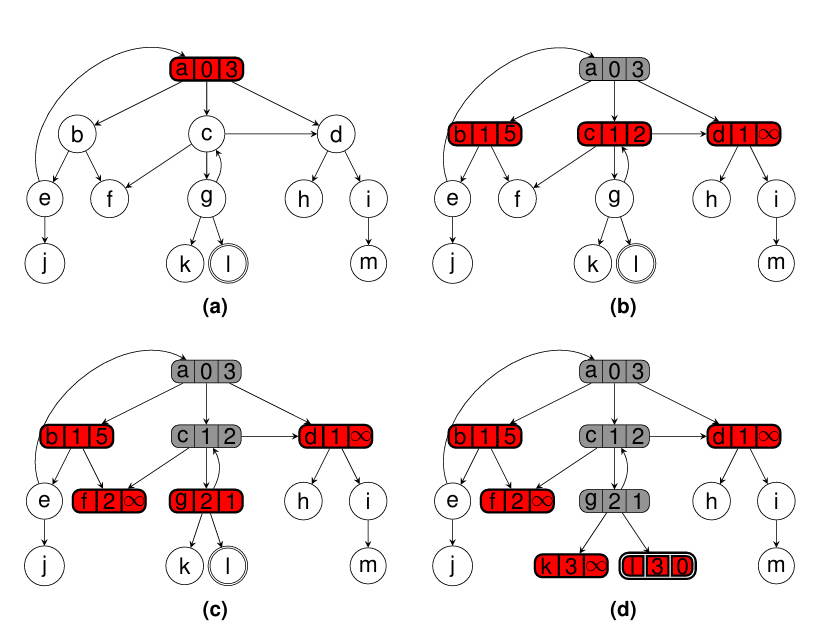
\includegraphics[width=0.8\textwidth]{./imgs/astar.png}
	\caption{A* Algorithm}
\end{figure}

\subsubsection{Pseudocode}
\begin{algorithm}[H]
	\caption{A* Search (\textit{start, goal, heuristic})}
	\label{alg:astar}
	\begin{algorithmic}[1]
		\State priority queue \(\gets\) [(start, cost = 0, estimated total cost = heuristic(start))]
		\While {priority queue is not empty}
		\State (node, cost) \(\gets\) dequeue(priority queue)
		\If {node = goal}
		\State return path
		\EndIf
		\ForAll {neighbor in valid moves}
		\State new cost \(\gets\) cost + move cost
		\State estimated total cost \(\gets\) new cost + heuristic(neighbor)
		\If {neighbor not visited or new cost \(<\) previous cost}
		\State mark neighbor as visited
		\State enqueue(priority queue, (neighbor, new cost, estimated total cost))
		\EndIf
		\EndFor
		\EndWhile
		\State return failure
	\end{algorithmic}
\end{algorithm}

\subsubsection{Implementation}
\begin{itemize}
	\item \textbf{\_\_init\_\_(\ldots)}
	      Initializes the A* search algorithm with grid dimensions, matrix representation, initial player position, stone positions, and switch positions. It also includes options for deadlock detection and heuristic optimization.

	\item \textbf{search()}
	      Implements the A* search algorithm using a priority queue (min-heap). The function explores states by selecting the one with the lowest cost \(f = g + h\). It expands nodes by generating successors, updating costs, and maintaining a hash table for efficient state lookup.

	\item \textbf{handle(new\_state, closed, frontier, state\_hash\_table)}
	      Manages newly generated states, checking if they should be added to the frontier or updated in the hash table based on their cost values.

	\item \textbf{heuristic(stones\_pos, switches\_pos)}
	      Computes the heuristic function to estimate the cost to reach the goal. It selects between the Hungarian heuristic and Manhattan heuristic based on the optimization flag.

	\item \textbf{mahattan\_heuristic(stones\_pos, switches\_pos)}
	      Calculates the heuristic using the Manhattan distance, summing up the minimum distances from each stone to a switch.

	\item \textbf{hungarian\_heuristic(stones\_pos, switches\_pos)}
	      Uses the Hungarian algorithm to optimally assign stones to switches, minimizing the total weighted Manhattan distance.

	\item \textbf{can\_go(current\_state, dir)}
	      Checks whether the player can move in a given direction from the current state without encountering obstacles.

	\item \textbf{go(current\_state, dir, heuristic)}
	      Generates a new state by moving the player in the specified direction, updating positions and recalculating heuristic values.

	\item \textbf{construct\_path(final\_state)}
	      Reconstructs the sequence of moves leading to the goal state by backtracking from the final state.

\end{itemize}

\subsubsection{Heuristics in A* Algorithm}
A* search uses a heuristic function \( h(n) \) to estimate the cost from a given state to the goal. The total cost function is defined as:
\[
f(n) = g(n) + h(n)
\]
where:
\begin{itemize}
    \item \( g(n) \) is the actual cost from the start state to the current state \( n \).
    \item \( h(n) \) is the estimated cost from \( n \) to the goal state.
\end{itemize}
For Sokoban, common heuristic choices include:
\begin{itemize}
    \item \textbf{Manhattan Distance:} The sum of the absolute differences between the x and y coordinates of each stone and its nearest goal position.
    \item \textbf{Hungarian Algorithm:} Computes an optimal assignment of stones to switches, minimizing the total weighted Manhattan distance.
\end{itemize}
A* is optimal if \( h(n) \) is \textit{admissible} (never overestimates the true cost) and \textit{consistent} (satisfies the triangle inequality).

\subsubsection{Time and Space Complexity}
\textbf{Time Complexity:} \( O(b^d) \) in the worst case, but with a good heuristic, it can be significantly reduced. If the heuristic is admissible and consistent, A* is optimal and complete.

\textbf{Space Complexity:} \( O(b^d) \), as it keeps all generated nodes in memory.
